\section{Исследовательский раздел}

В данном разделе проводится параметризация выбранных алгоритмов векторизации, понижения размерности и модели нечеткой кластеризации. Проведено сравнение модели Гауссовой смеси собственной реализации и модели из библиотеки scikit-learn \cite{GMM}. Также приведены эксперименты, на основе которых были выбраны наиболее оптимальные параметры для решения данной задачи.

\subsection{Выборка данных}

Датасет собран из новостей на английском языке с сайта MSN.com. \cite{msn}

На вход векторизатору подается выборка данных размером 98247 документов, каждая из которых представляет собой предобработанную строку на английском языке, а также дату публикации.

Данные хранятся в файле имеющем формат tsv --- это формат для представления таблиц баз данных. Для последующего обучения модели нечеткой кластеризации использовалась полная выборка данных, так как каждой новости требуется сопоставить кластер для корректной работы алгоритма.

\subsection{Сравнение методов}

В данном разделе будет произведено сравнение собственной реализации модели Гауссовой смеси и модели из библиотеки scikit-learn. Будет создан искусственный набор данных имеющий 3 кластера. После выполнения кластеризации собственным методом и методом из библиотеки scikit-learn будет произведена оценка кластеризации V-мерой, которая представляет из себя гармоническое среднее оценки однородности и полноты.

На рисунке \ref{Clust_0} приведен исходный размеченный набор данных размером 400, а на рисунках \ref{Clust_1} и \ref{Clust_2} приведен набор данных кластеризованный собственным методом Гауссовой смеси и методом из библиотеки scikit-learn.

\begin{figure}[H]
	\centering
	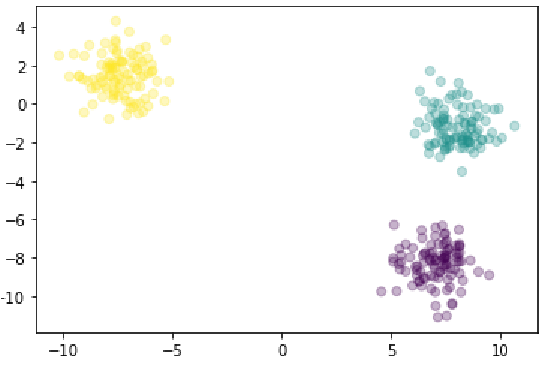
\includegraphics[width=\textwidth]{img/Clust_0.pdf}
	\caption{График исходного набора данных. Цветами выделены кластеры.}
	\label{Clust_0}
\end{figure}  

\begin{figure}[H]
	\centering
	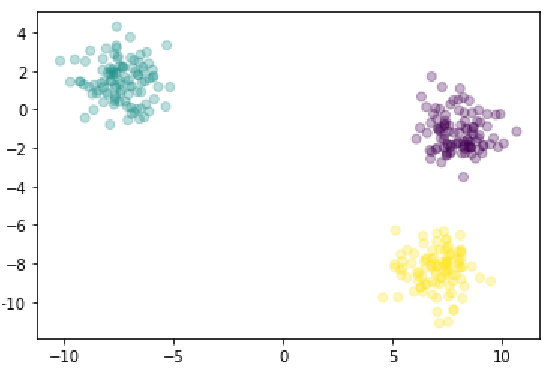
\includegraphics[width=\textwidth]{img/Clust_1.pdf}
	\caption{График набора данных, кластеризованный собственным методом Гауссовой смеси.}
	\label{Clust_1}
\end{figure}  

\begin{figure}[H]
	\centering
	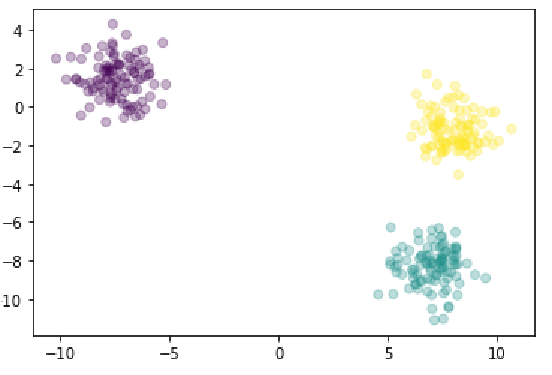
\includegraphics[width=\textwidth]{img/Clust_2.pdf}
	\caption{График набора данных, кластеризованный методом Gaussian Mixture Model из библиотеки scikit-learn.}
	\label{Clust_2}
\end{figure}

Как можно заметить алгоритм собственной реализации корректно разделяет данные. Заключительным этапом является оценка кластеризации V-мерой, результат оценки приведен в таблице \ref{measure_table}

\begin{table}[H]
	\caption{Сравнение реализованного метода Гауссовой смеси с методом из библиотеки scikit-learn}
	\label{measure_table}
	\begin{center}
		\begin{tabularx}{1\textwidth}{ 
				| >{\raggedright\arraybackslash}X 
				| >{\centering\arraybackslash}X 
				| >{\centering\arraybackslash}X | }
			\hline
			Количество образцов & Значение V-меры реализованного метода & Значение V-меры метода из scikit-learn \\ 
			\hline
			100 & 0.930 & 0.965 \\ 
			\hline
			250 & 0.930 & 0.930 \\ 
			\hline
			300 & 0.940 & 0.965 \\  
			\hline
		\end{tabularx}
	\end{center}
\end{table}

Как можно заметить по таблице, метод собственной реализации лишь незначительно уступает в точности методу из библиотеки scikit-learn, а при значении 2500 совпадает.

\subsection{Порядок параметризации}

Для достижения наилучшего качества нечеткой кластеризации и последующих рекомендаций в первую очередь следует определить оптимальные параметры векторизатора TF-IDF, после чего требуется определить оптимальное количество компонентов, которые следует оставить для того, чтобы доля объясненной дисперсии после понижения размерности была не меньше 0.95. Заключительным этапом является подбор оптимальных параметров модели Гауссовой смеси для достижения наилучшего качества.

\subsubsection{Параметризация векторизатора TF-IDF}

Для получения наилучших параметров векторизатора будем варьировать максимальную величину параметра DF (документная частота, то есть максимальное допустимое число документов, в которых встретился термин t), термины выше порогового значения не будут использоваться при векторизации, также будет варьироваться диапазон N-грамм, то есть будут ли признаки формироваться из отдельных слов или из нескольких.

Качество векторизатора будем проверять с помощью оценки последующей нечеткой кластеризации мерой Силуэт. Параметры метода понижения размерности и нечеткой кластеризации заданы по умолчанию. Результат исследования приведен на таблице \ref{vectorizer_comp_table}.

\begin{table}[H]
	\caption{Значение критерия Силуэт от параметров векторизатора TF-IDF}
	\label{vectorizer_comp_table}
	\begin{center}
		\begin{tabularx}{1\textwidth}{ 
				| >{\raggedright\arraybackslash}X 
				| >{\centering\arraybackslash}X 
				| >{\centering\arraybackslash}X | }
			\hline
			\diagbox[width=11em]{$Max\_df$}{используемые\\n-граммы} & Слова по отдельности & Слова по отдельности и пары слов \\ 
			\hline
			0.25 & 0.912 & 0.923 \\ 
			\hline
			0.30 & 0.905 & 0.919 \\ 
			\hline
			0.35 & 0.903 & 0.918 \\  
			\hline
		\end{tabularx}
	\end{center}
\end{table}

Посмотрев на таблицу выше можно сделать вывод о том, что наилучшими значениями параметров векторизатора являются 0.25 для параметра $max\_df$ и использование как всех слов по отдельности так и пар слов.

\subsubsection{Параметризация метода понижения размерности SVD}

Так как исходная выборка обладает большой размерностью, а также является разреженной требуется применить метод понижения размерности в целях экономии памяти и увеличения скорости работы. Целевым показателем является доля объясненной дисперсии, ее значение должно равняться не менее 0.95.

На рисунке \ref{ExpVariance} приведена зависимость количества компонентов после понижения размерности и долю объясненной дисперсии для данного количества компонент.

\begin{figure}[H]
	\centering
	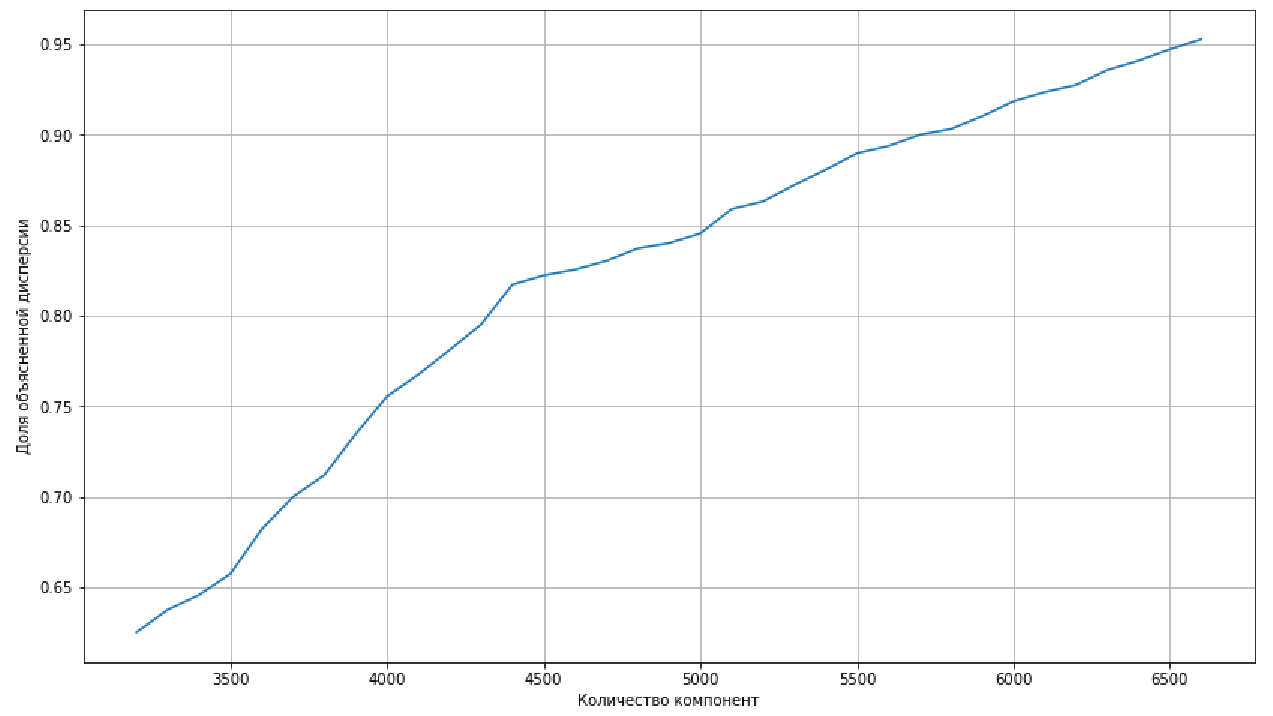
\includegraphics[width=\textwidth]{img/ExpVariance.pdf}
	\caption{Доля объясненной дисперсии в зависимости от количества компонент.}
	\label{ExpVariance}
\end{figure}  

Как можно заметить на картинке вышее необходимое количество компонент составляет 6700, при данном количество доля объясненной дисперсии составляет чуть выше 0.95. Данный этап позволил сохранить информативность данных и сэкономил большой количество ресурсов памяти.

\subsubsection{Параметризация метода Гауссовой смеси}

Для достижения наилучшего результата нечеткой кластеризации требуется варьировать ключевой параметр, которым является количество кластеров, требуется получить такое количество кластеров при котором оценка методом Силуэта будет давать наивысший результат (быть как можно более близким к 1). Для достижения необходимого результата был проведен эксперимент при котором варьировалась количество кластеров. Зависимость полученной оценки от количества кластеров можно увидеть на рисунке \ref{SilhScore}

\begin{figure}[H]
	\centering
	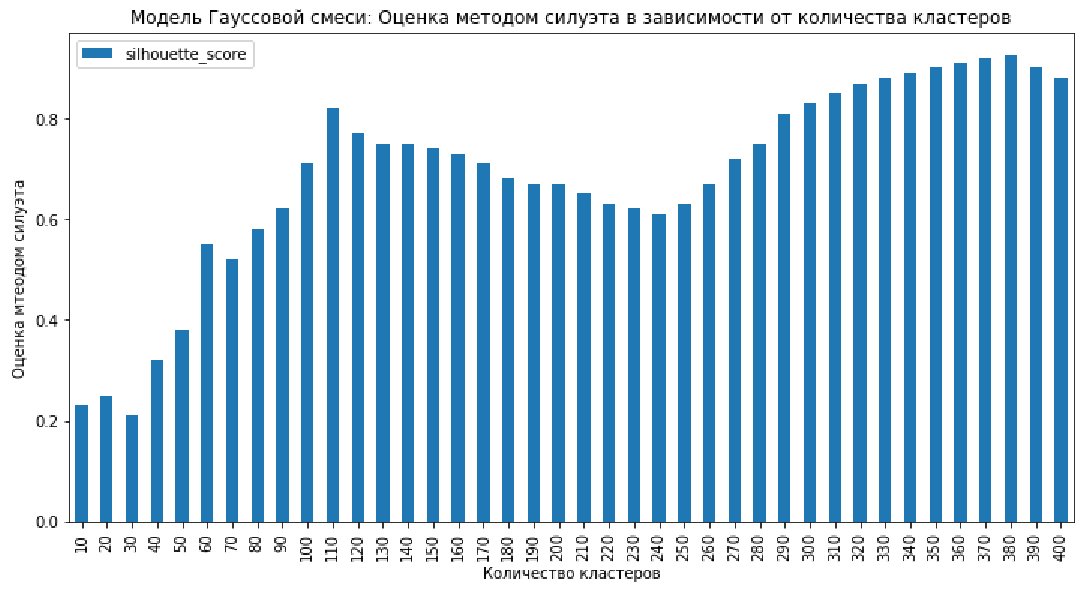
\includegraphics[width=\textwidth]{img/SilhScore.pdf}
	\caption{Полученная оценка методом Силуэта в зависимости от количества кластеров.}
	\label{SilhScore}
\end{figure}  

Видно, что явные пики на графике это 110 кластеров и 380 кластеров. При количестве кластеров равным 380 оценка достигает порядка 0.92 по методу силуэта, что является очень хорошим показателем, именно данное количество кластеров и было использовано при построении финальной версии рекомендательной системы.

\subsection{Рекомендации к применению рекомендательной системы}

После проведения исследования и параметризации, полученной рекомендательной системы можно сделать вывод о том, что она работает эффективно и исправно. Данную систему можно применять при создании собственных новостных сайтов, но стоит учесть, что первоначальное обучение модели на уже имеющихся данных должно выполняться на мощной машине и кластеры новостям должны быть определены заранее, поскольку векторизатор, метод понижения размерности и сама нечеткая кластеризация методом Гауссовой смеси являются трудоемкими операциями в случае большого объема данных.

\subsection{Выводы из исследовательского раздела}

В данном разделе была проведена парметризация алгоритмов из ключевых этапов построения рекомендательной системы, а также проведена проверка качества работы разработанного метода в сравнении с методом из библиотеки scikit-learn с помощью V-меры, в ходе которой было выявлено, что разработанный метод в большинстве случаев не уступает методу из библиотеки. Параметризовав алгоритм векторизации был сделан вывод о том, что наилучшим значением для параметра $max_df$ векторизатора Tf-IDF является 0.25, а в качестве n-грамм следует брать как слова по отдельности так и пары слов. Для метода понижения размерности наилучшим количеством компонент является 6700, поскольку доля объясненной дисперсии при данном количестве превышает 0.95, что очень хорошо описывает данные, экономя при этом память. Заключительным этапом было выявление оптимального количества кластеров в модели Гауссовой смеси, в качестве результата была получена зависимость оценки метода Силуэта от количества кластеров, исходя из которой можно сделать вывод о том, что наилучшее количество кластеров для построения рекомендательной системы на исходных данных равно 380. В конце данного раздела была описана применимость разработанной рекомендательной системы.

\pagebreak